\chapter{Resultat}
I denna delen kommmer resultatet av projekt beskrivas. Det innebär dels
resultate på den mjukvara som ha utvecklats men även vilka erfarenheter som
teamet har samlat på sig under projektets gång.
\section{Systembeskrivning}
\textit{Skrivs när systemet är byggt, vill man få en känsla för hur det kan
komma att se ut så läser man bäst om det i arkitekturdokumentet}
\section{Prototyper}
Under projektets andra iteration så togs tre olika prototyper fram. Dessa
prototyper designades för att visa på olika designalternativ på
användargränssnittet. Ett exempel på detta är informationen som var med i listan
över beslutade operationer. I en av prototyperna identifierades patienten som hörde
ihop med beslutet med namn i den andra med personnummer. I den tredje prototypen
fanns inget alls som identifierade patienten utan enbart information om vilken
typ av operation det var. På liknande sätt utvärderades olika sätt att
visualisera lediga tider i schemat samt olika sätt att anpassa sökparametrarna i
en sökning efter lediga tider. När prototyperna visades för kunden kunde
del olika alternativen sållas bort och en tydligare bild av behoven framträdde.
Till exempel beslutades att namn på patienten i samband med beslut var tydligast.

Den första iterationen av prototyper användes sedan för att ta fram en ny
prototyp med enbart mindre designalternativ som visades för tre olika
operationsplanerare.....
\textit{Detta kommer i nästa iteration}
\section{Systemanatomi}
\todo{referens samt bild på systemanatomi}
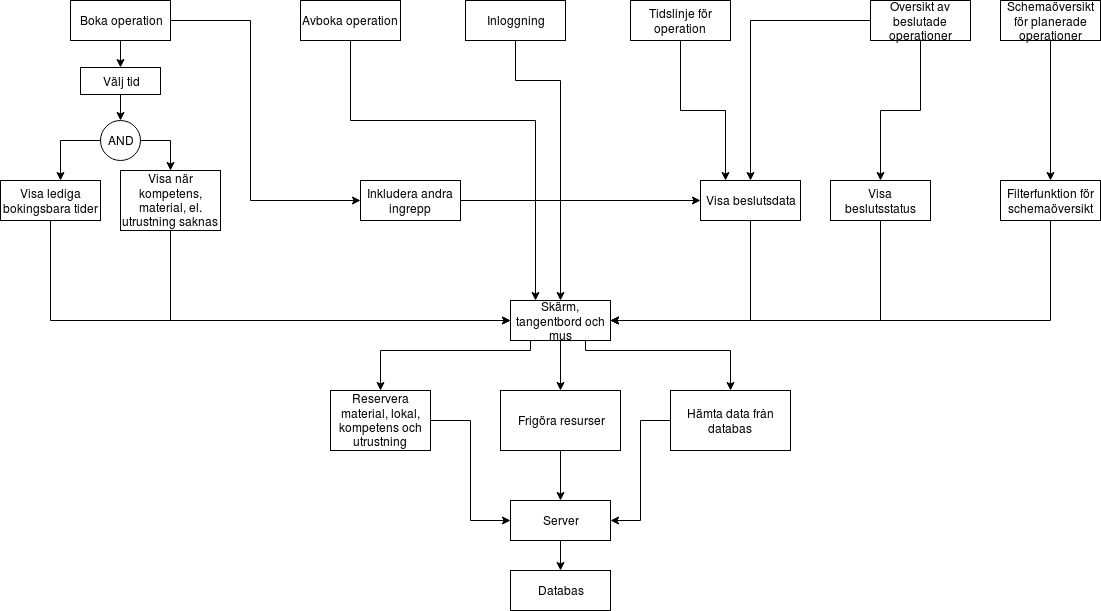
\includegraphics[width=\textwidth,height=.7\textheight]{Figures/Systemanatomi.png}\\

I första iterationen så togs det fram en systemanatomi som använts under
projektets gång för att styra arbetet under utvecklingen.


\section{Gemensamma erfarenheter}
I början av projektet så fick vi snabbt större erfarenhet av olika områden
tack vare de olika presentationer som de olika deltagarna i projektet hade.
Vi fick även en ökad förståelse för hur sjukvården fungerar och att ett bra
it-system kan göra verklig skillnad.

\section{Översikt över individuella bidrag}
I denna delen presenteras deltagarnas individuella bidrag översiktligt.

\todo{Lägg till era rubriker och en kort synopsis här}
\subsection{Adam}
Teamledarens roll kombinerat med scrum-metodik.
\subsection{Björn}
Hur kan versionshantering användas effektivt för ett mindre mjukvaruutvecklings projekt.
\subsection{Christoffer}
Betydelsen av att samla krav från en varierad grupp aktörer
\subsection{Henrik}
För/nackdelar med TypeScript jämfört med JavaScript
\subsection{Martin}
Angular som webbutvecklingsplattform
\subsection{Niclas}
Pappersprototypens betydelse vid utveckling av programvara
\subsection{Tor}
